\section{Error Analysis of Structured Light}
\frame{
  \frametitle{An Error Analysis of Structured Light Scanning of Biological Tissue}
  Sebastian Nesgaard Jensen, Jakob Wilm, Henrin Aanæs

  SCIA 2017
  \begin{figure}
    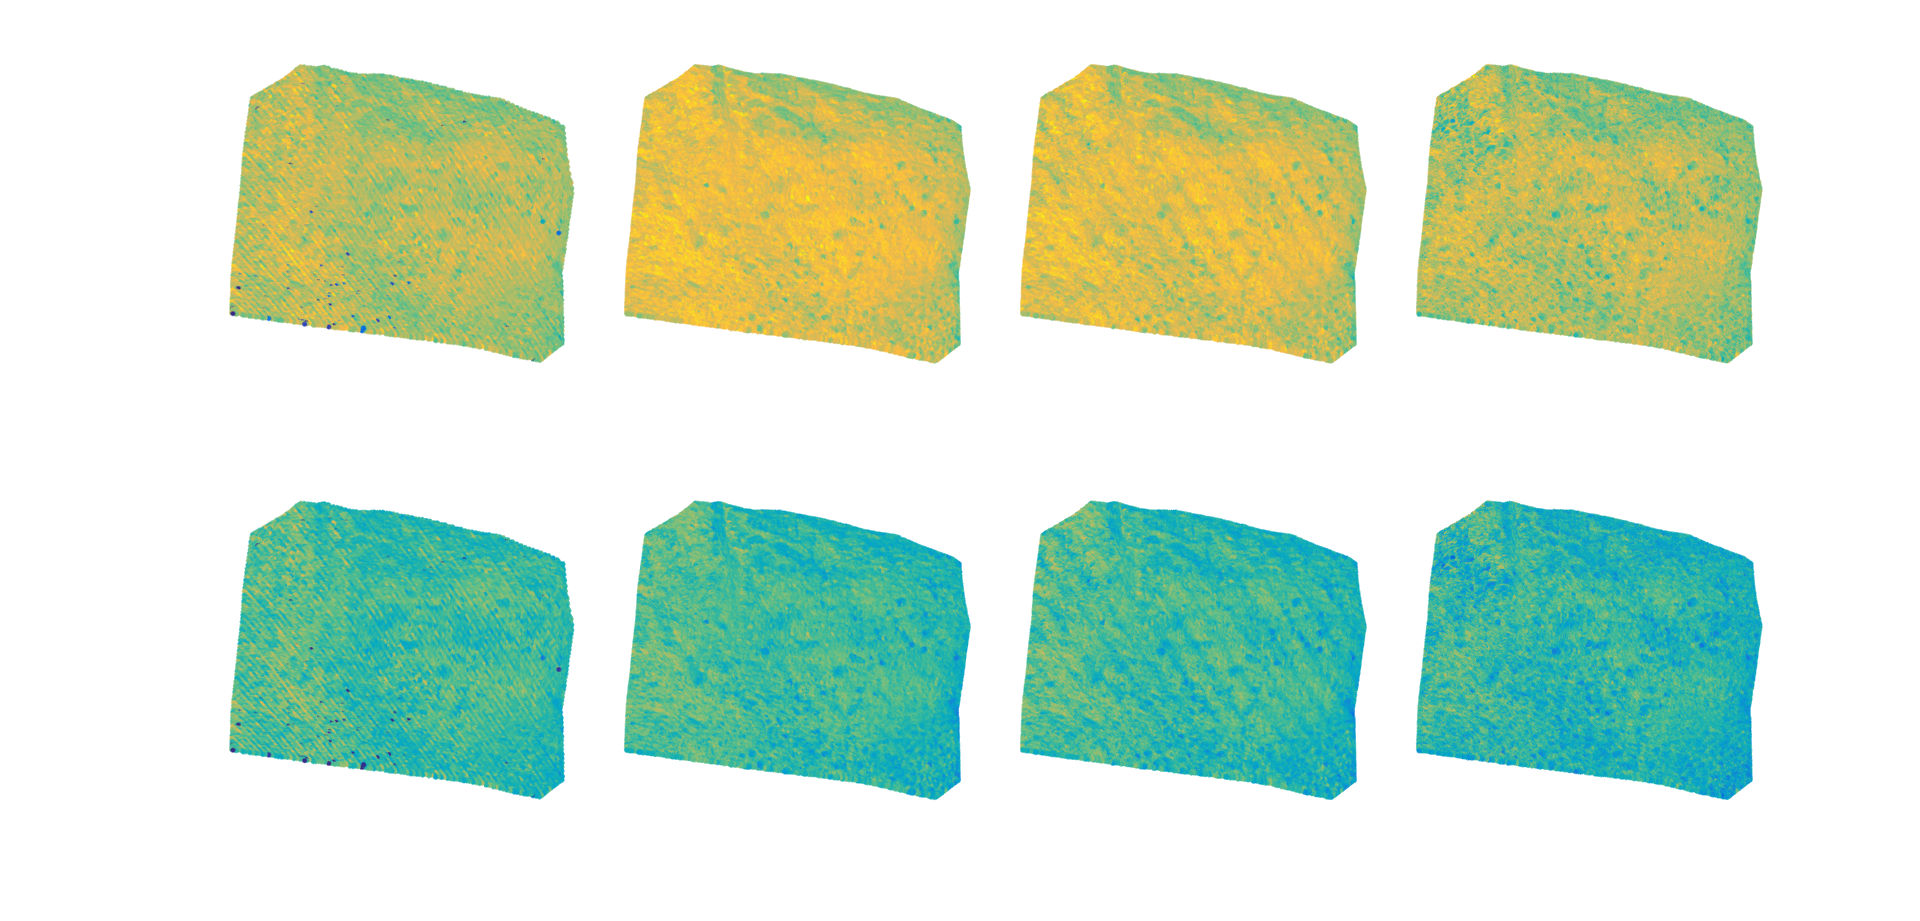
\includegraphics[width=0.80\linewidth]{figures/stlmeat}
      \hfill
  \end{figure}
  %\bibentry{jensen2017error}
}

\frame{
  \frametitle{Basic Ray Model}
  \begin{onlyenv}<1>
    \begin{figure}
      \centering
      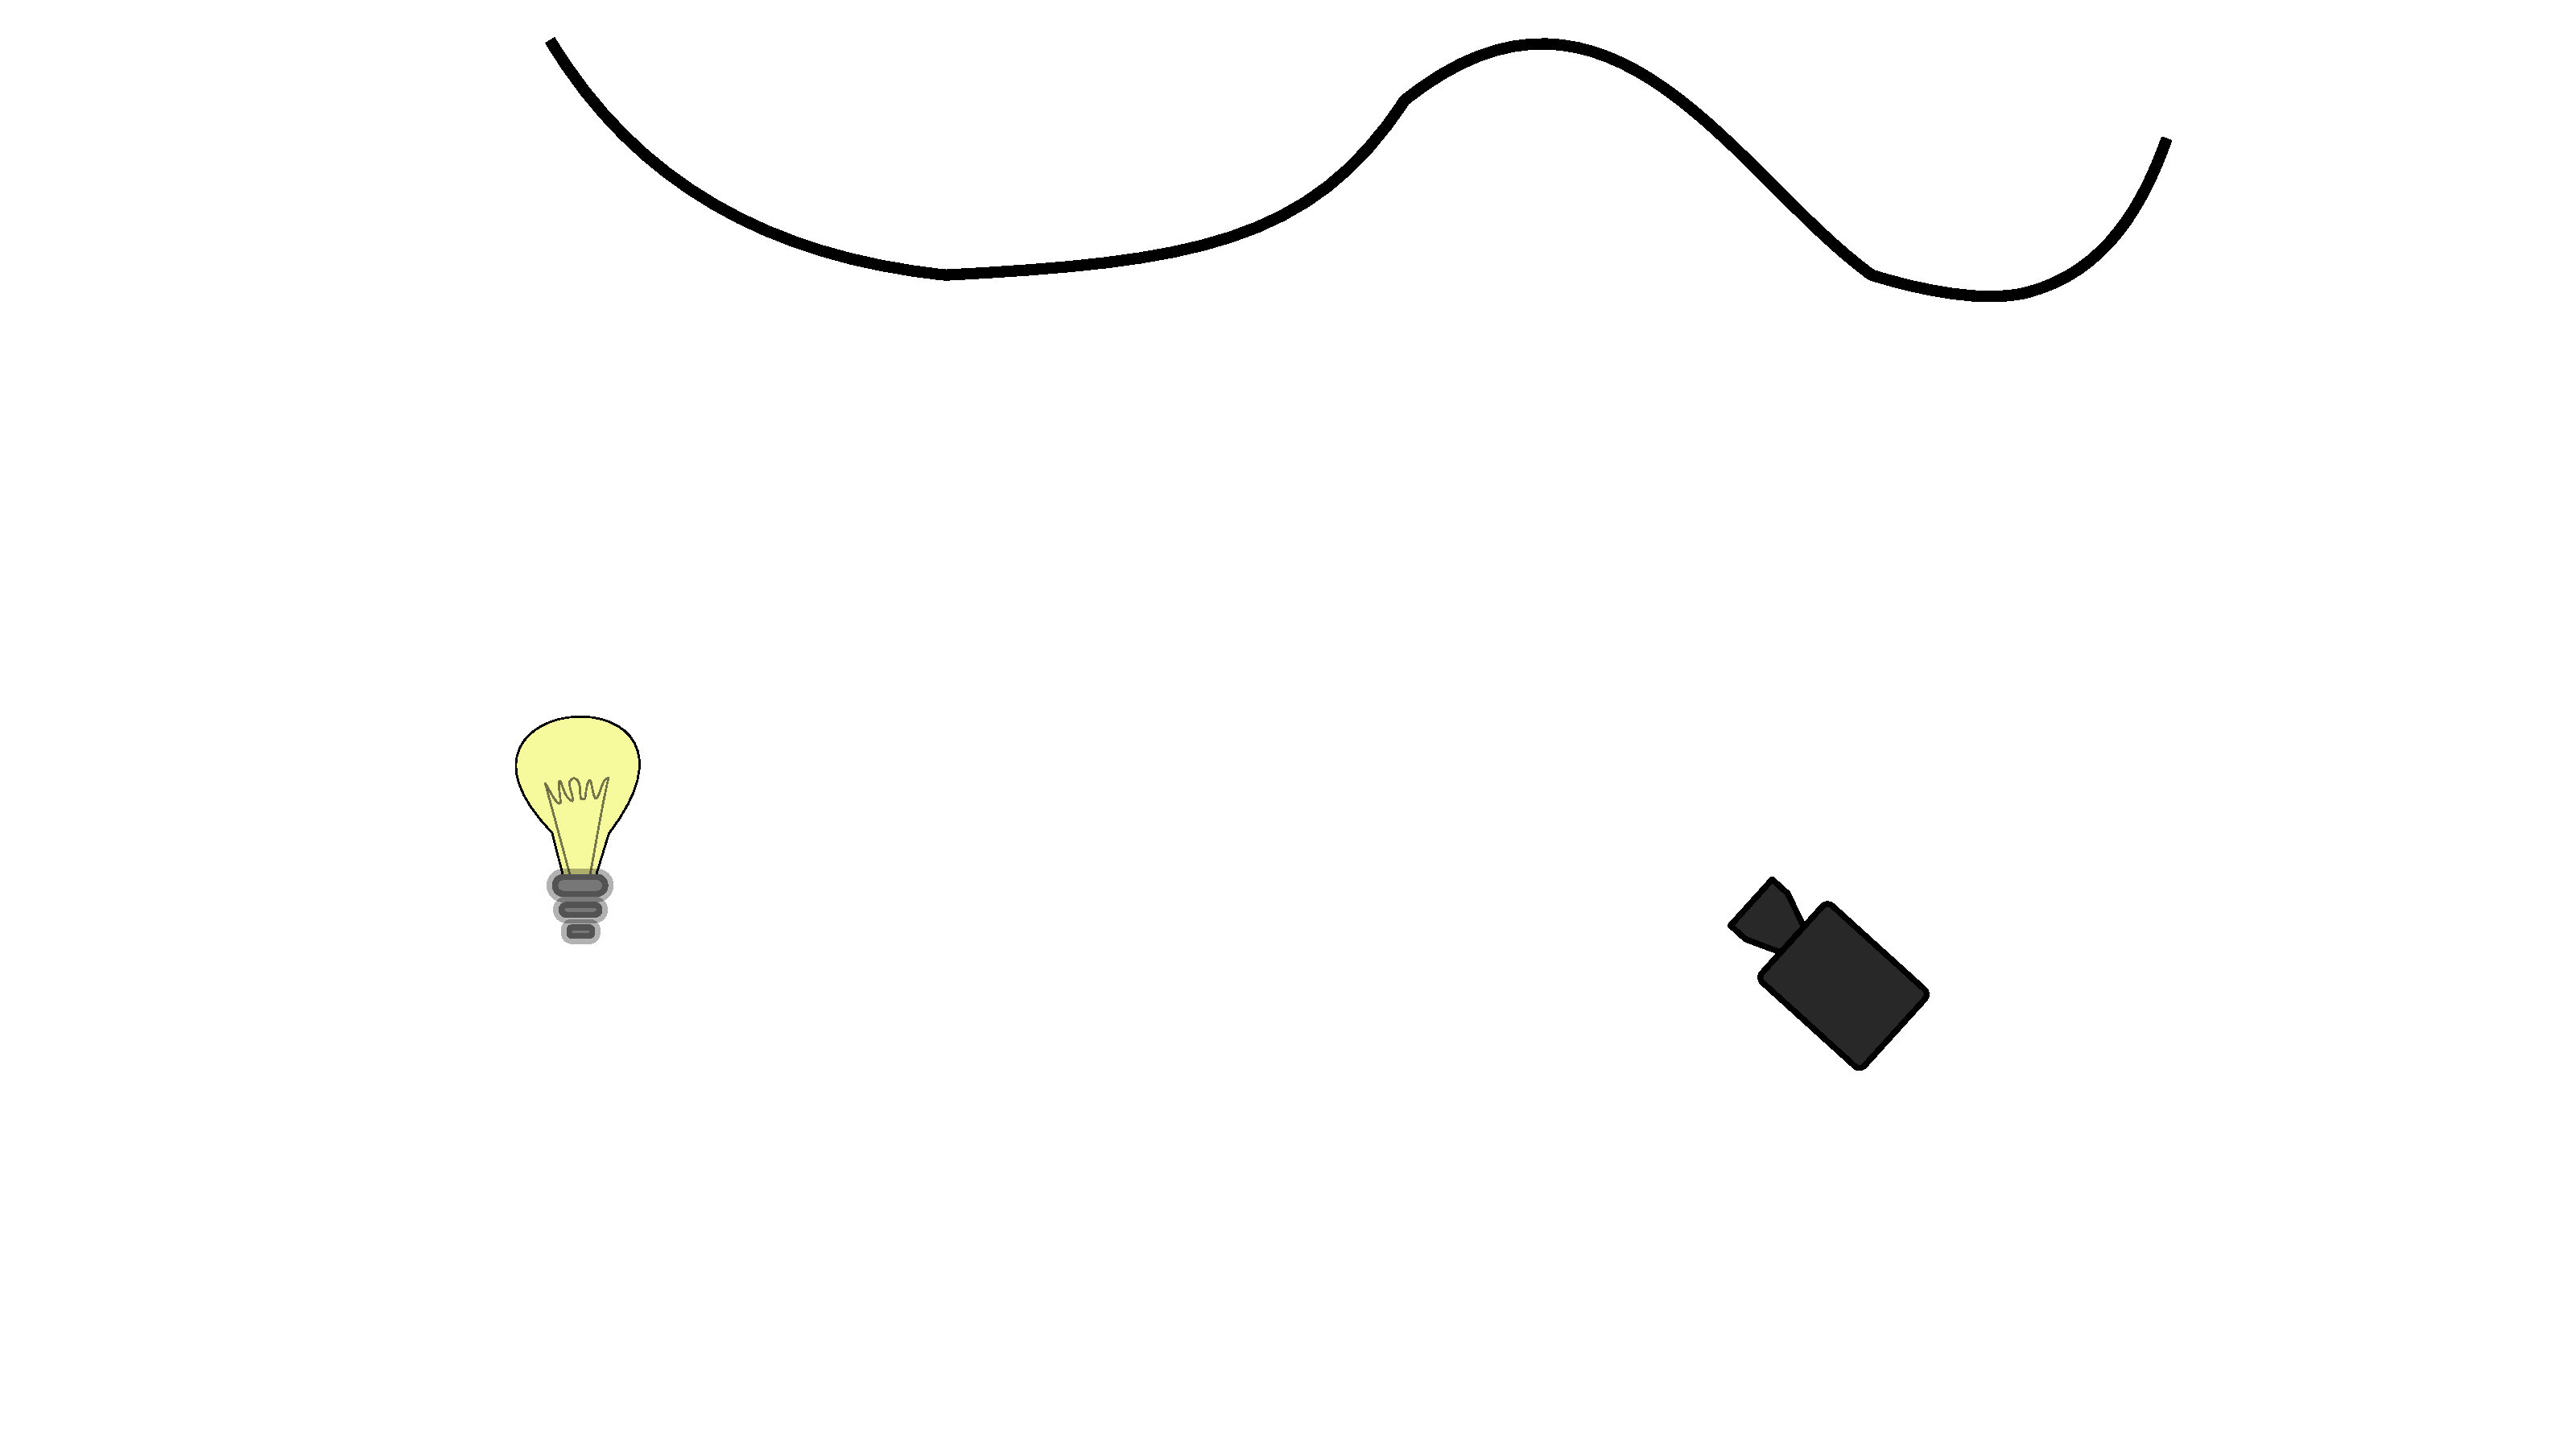
\includegraphics[width=0.8\linewidth]{figures/stl_none}
    \end{figure}
  \end{onlyenv}
  \begin{onlyenv}<2>
    \begin{figure}
      \centering
      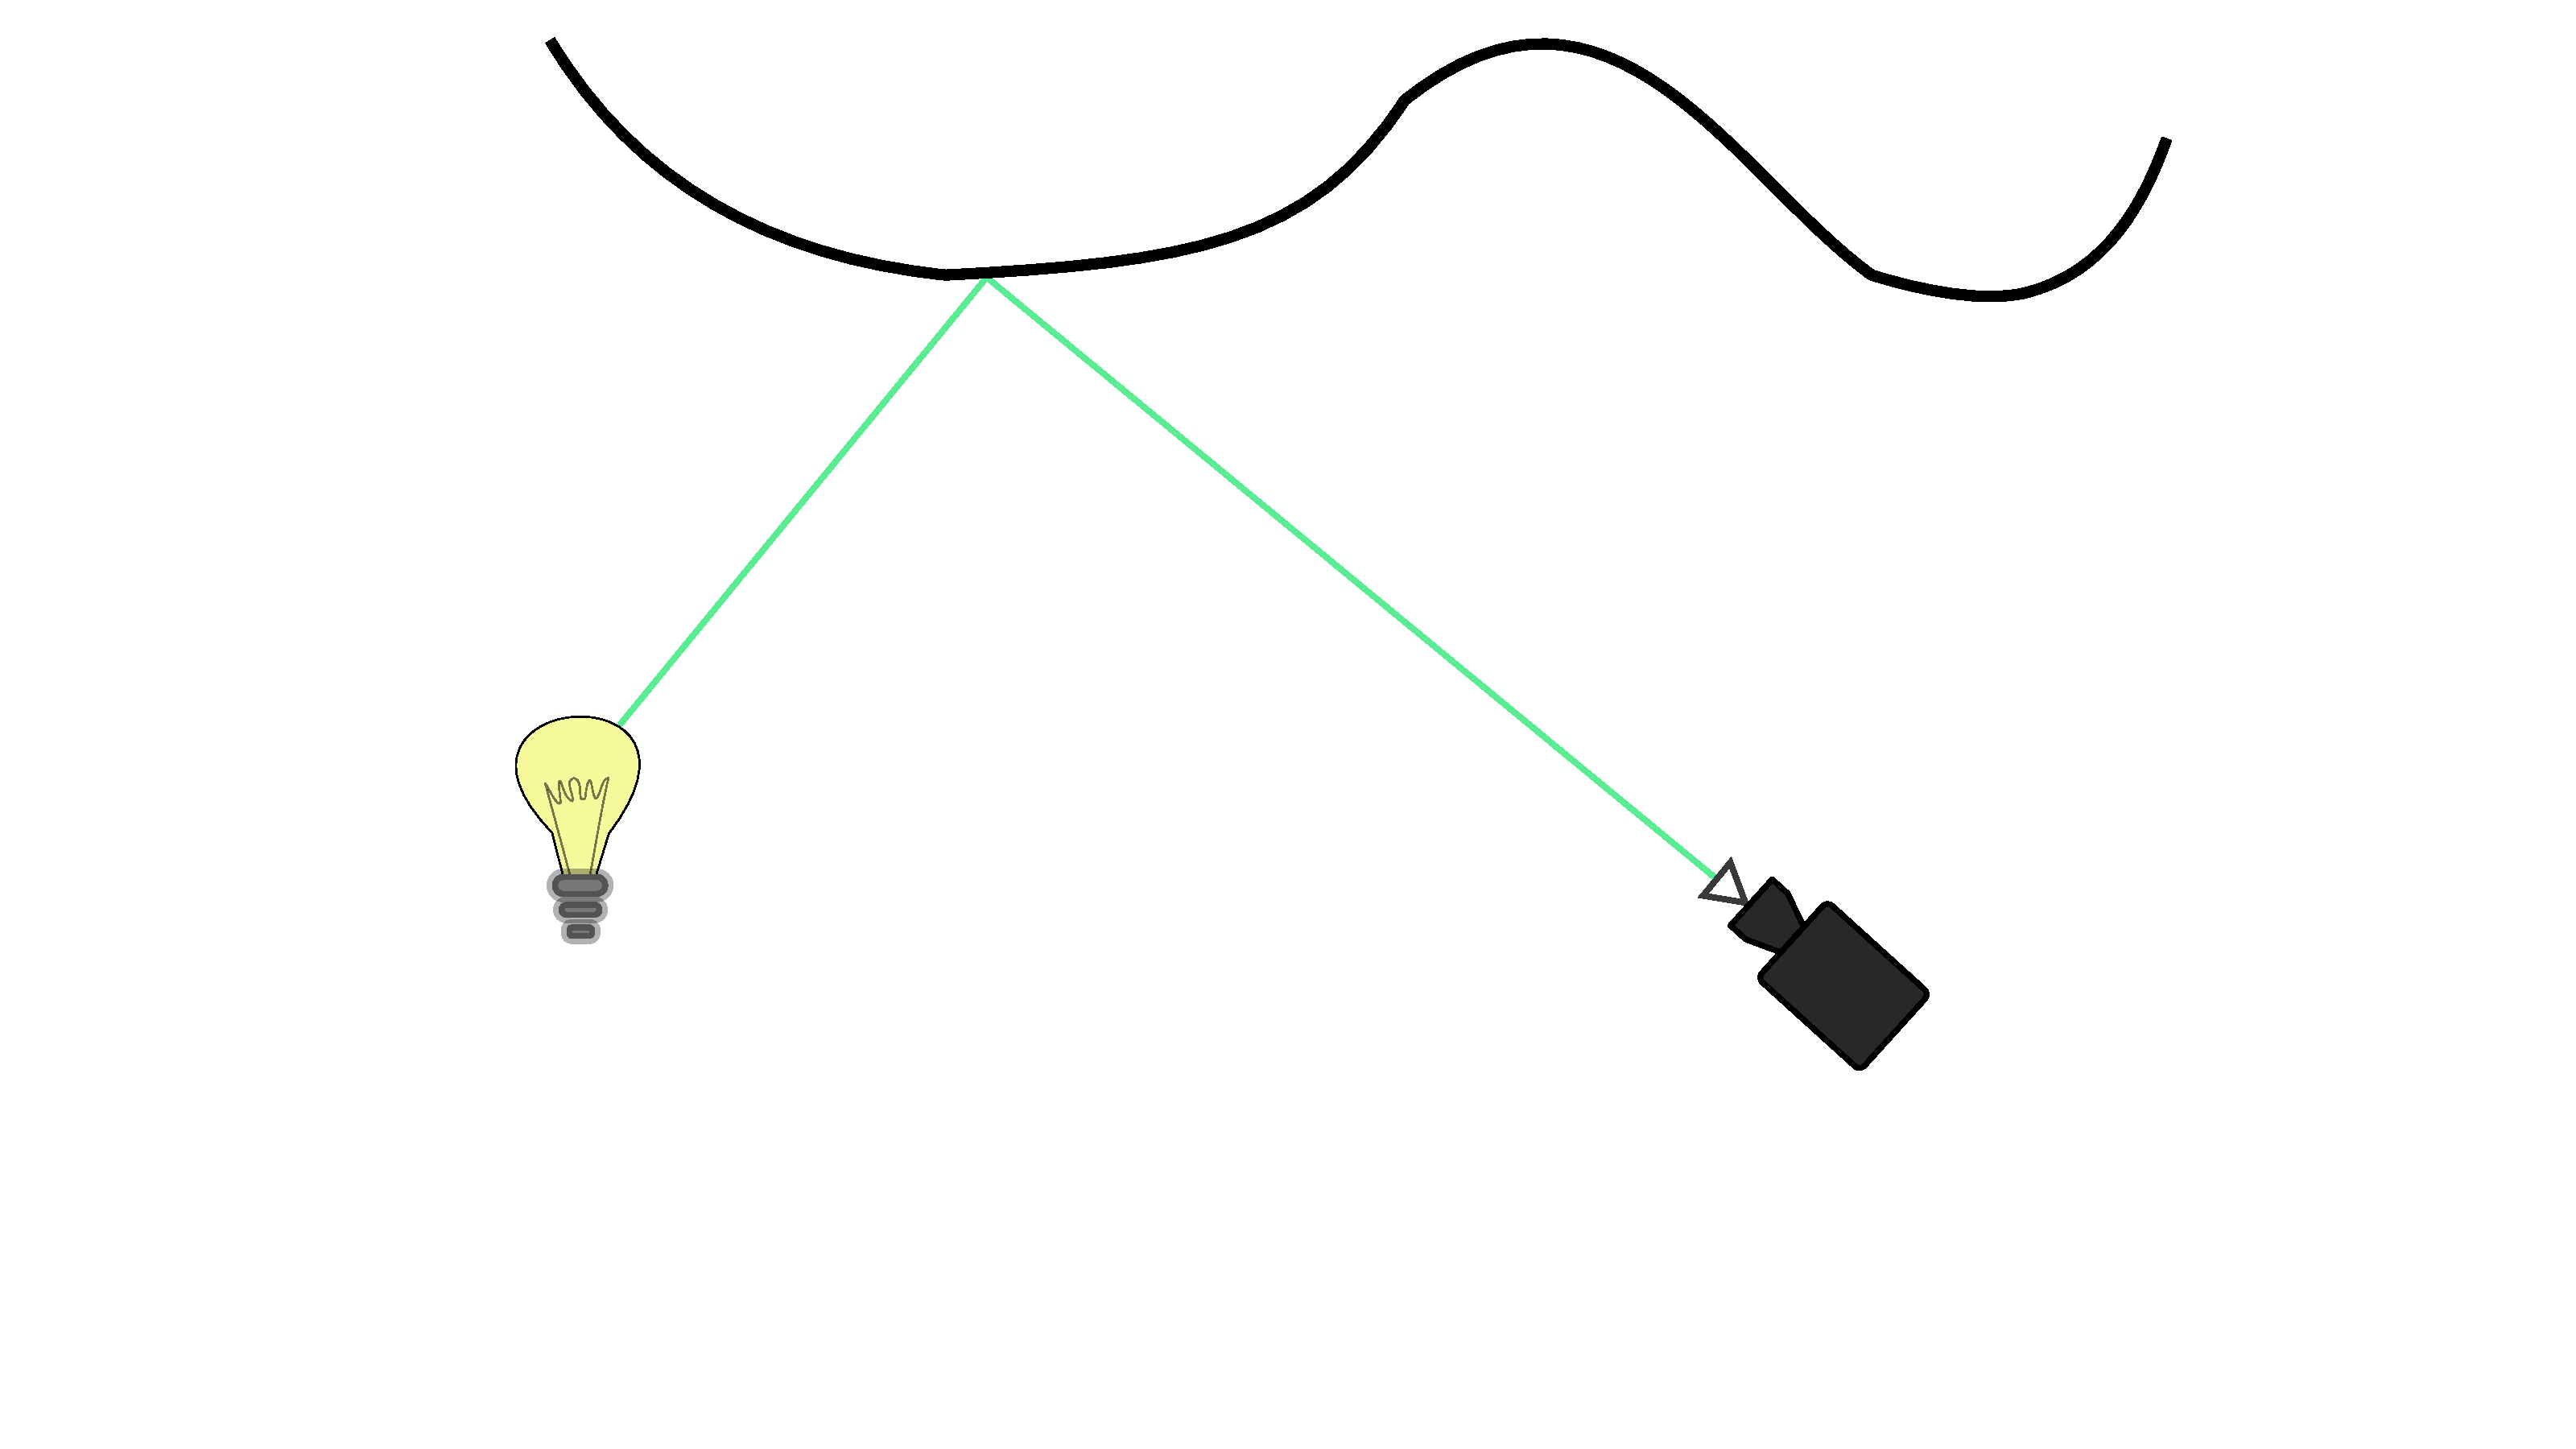
\includegraphics[width=0.8\linewidth]{figures/stl_direct}
    \end{figure}
  \end{onlyenv}
  \begin{onlyenv}<3>
    \begin{figure}
      \centering
      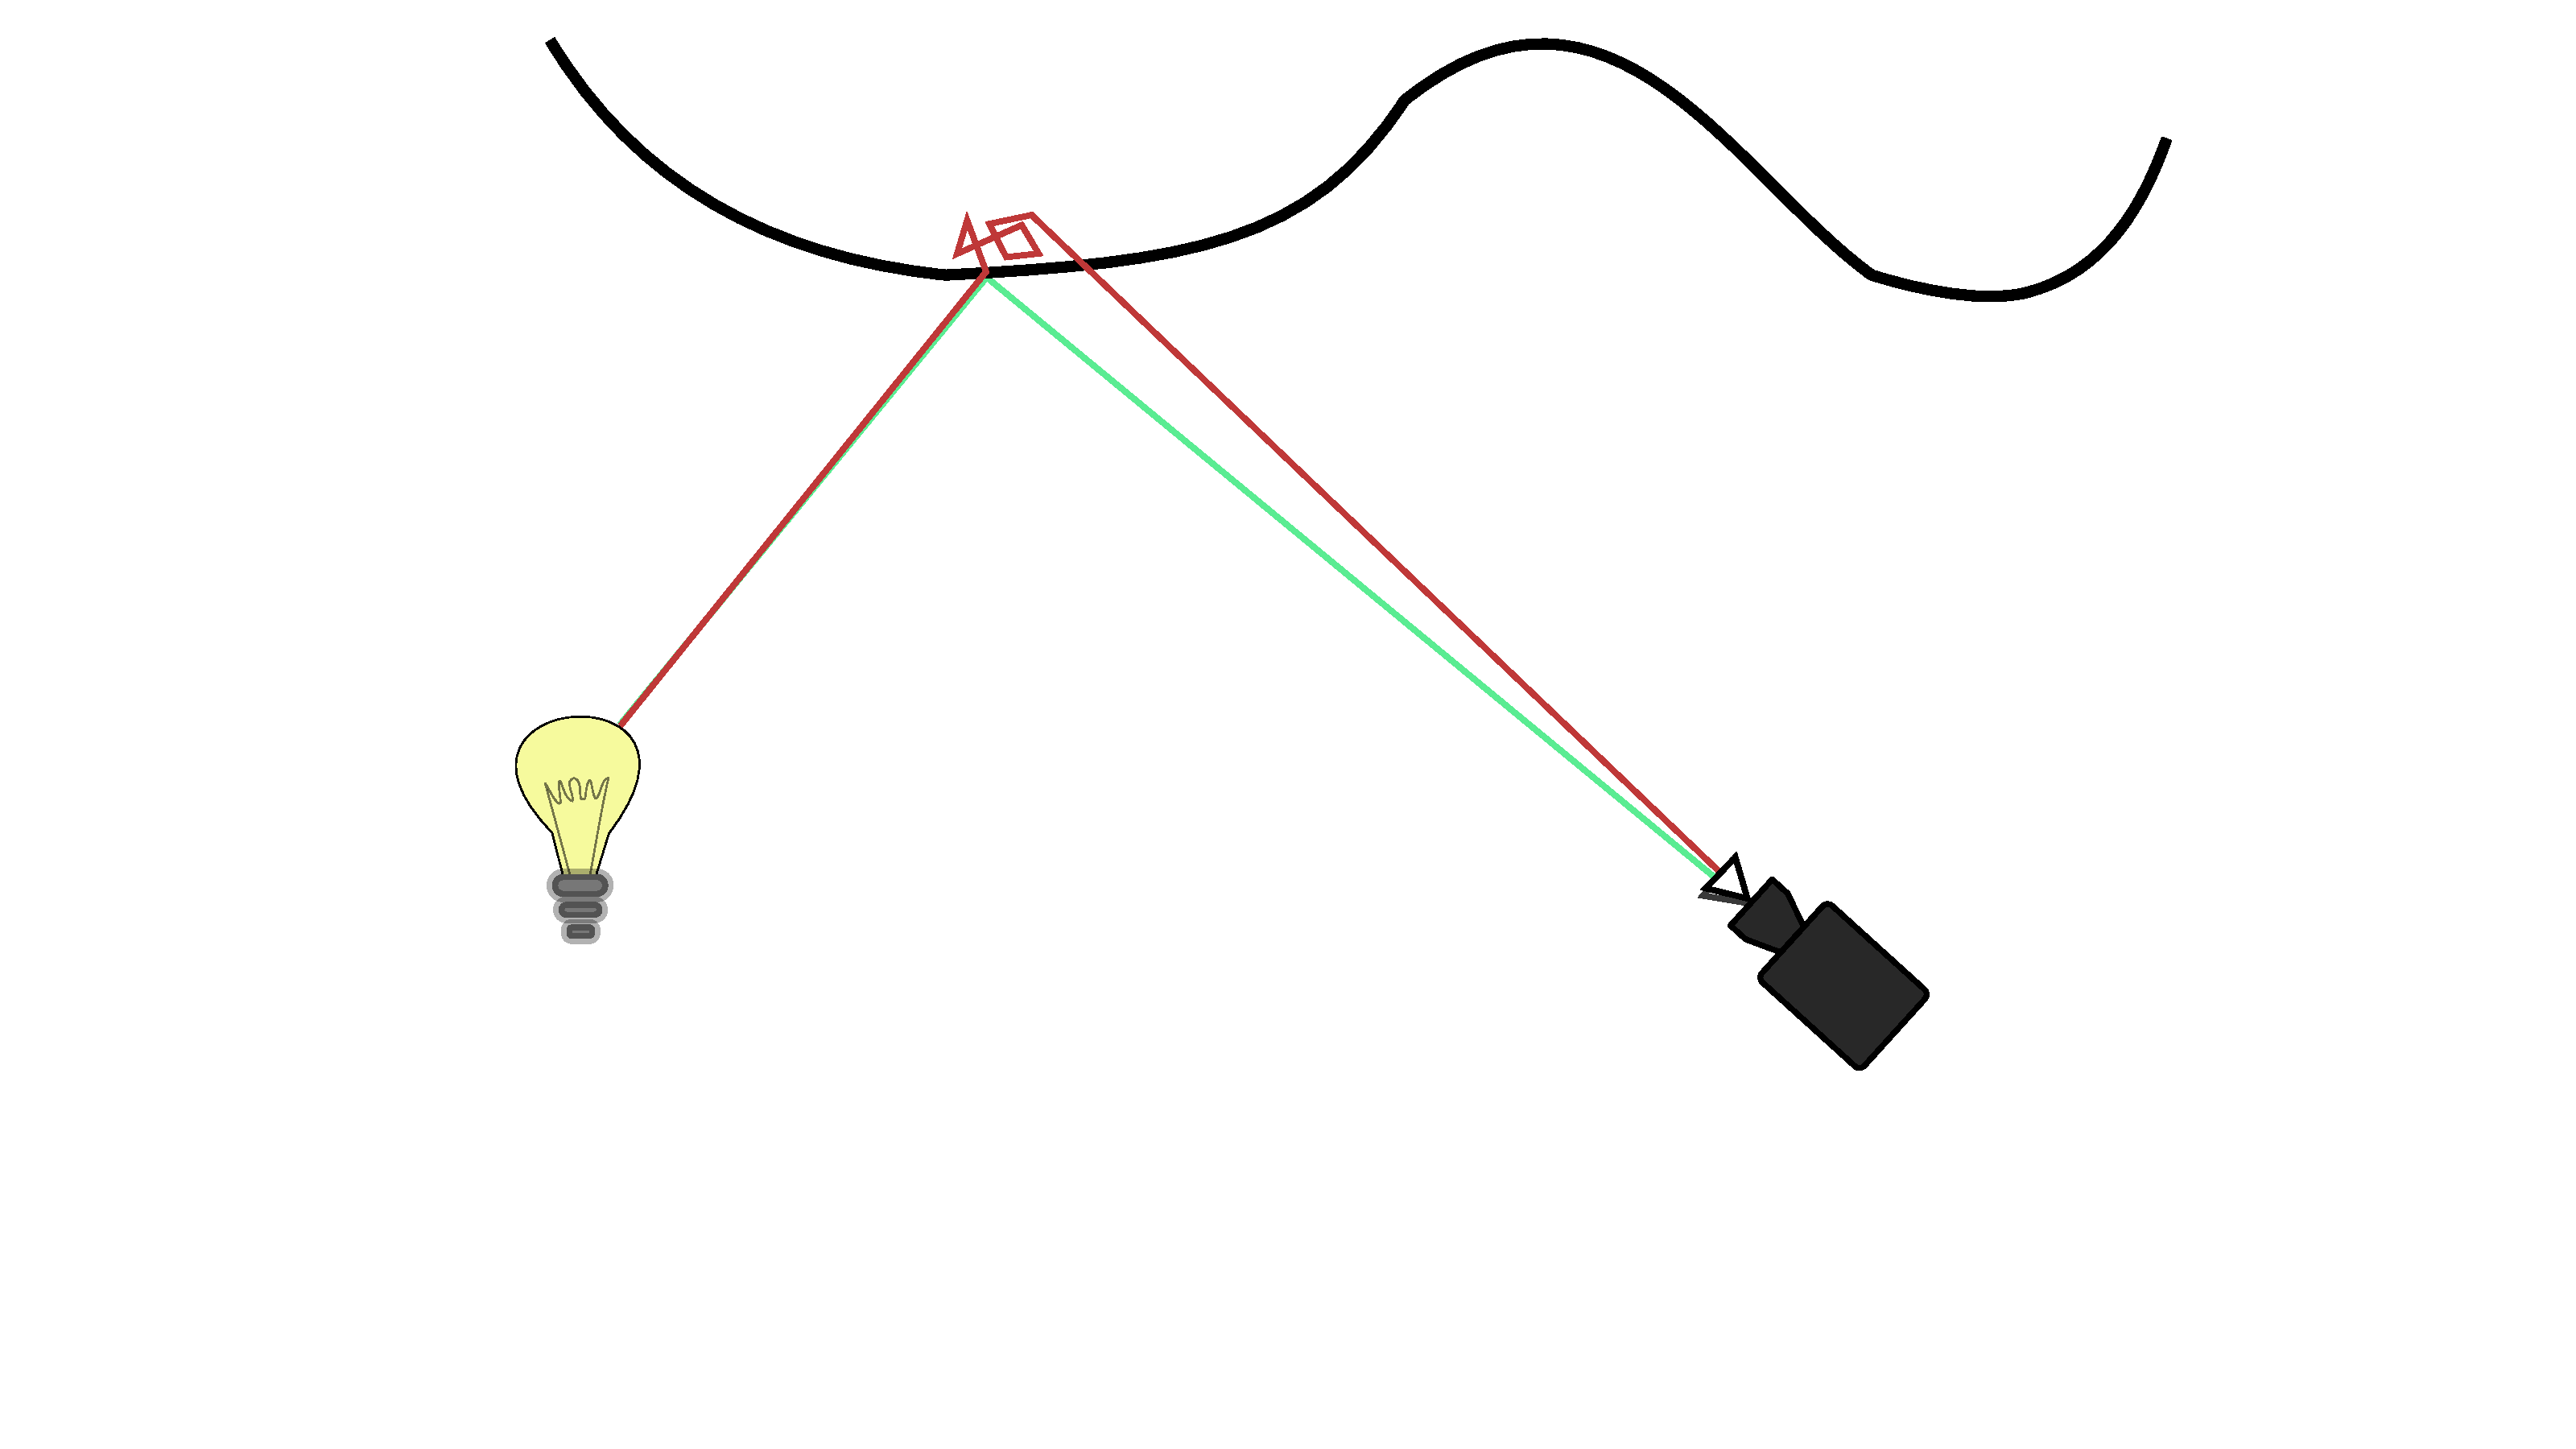
\includegraphics[width=0.8\linewidth]{figures/stl_all}
    \end{figure}
  \end{onlyenv}
}


\frame{
  \frametitle{Significance of Subsurface Scattering}
  \begin{figure}
    \centering
    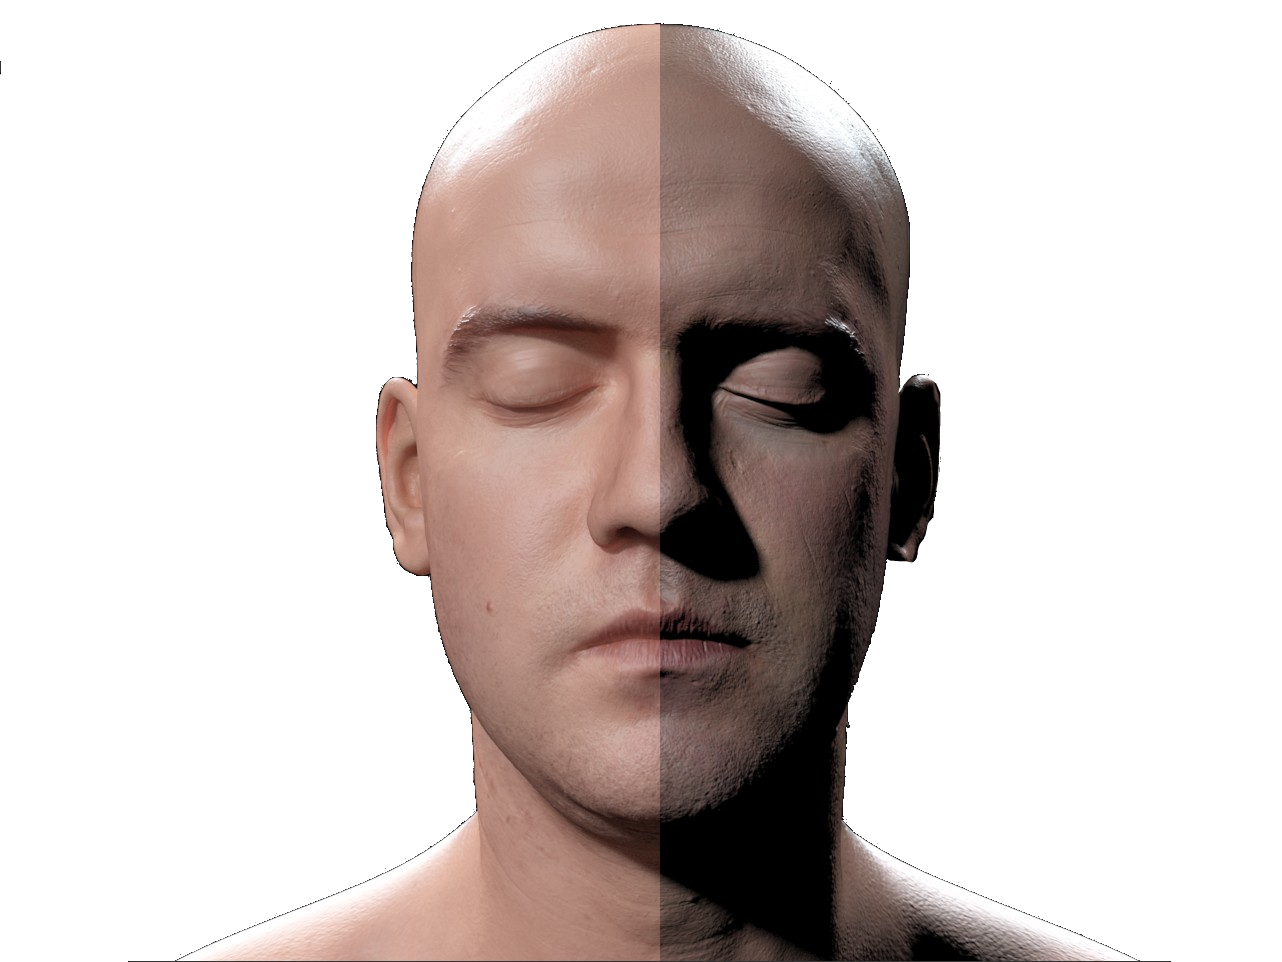
\includegraphics[height=0.8\textheight]{figures/humanss}
  \end{figure}
}

\frame{
  \frametitle{Materials and Structured Light Methods}
  \begin{minipage}[t]{0.48\linewidth}
    \captionsetup[subfloat]{position=above, labelformat=empty}
    \begin{figure}
      \subfloat[Skin]{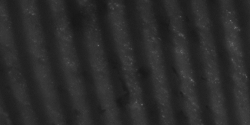
\includegraphics[width=0.49\linewidth]{figures/stlskinraw}}\hfill
      \subfloat[Fat]{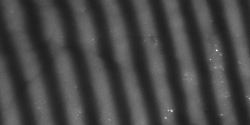
\includegraphics[width=0.49\linewidth]{figures/stlfatraw}}
    \end{figure}
    \captionsetup[subfloat]{position=below, labelformat=empty}
    \vspace{-1cm}
    \begin{figure}
      \subfloat[Meat]{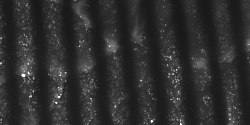
\includegraphics[width=0.49\linewidth]{figures/stlmuscleraw}}
    \end{figure}
  \end{minipage}\hfill
  \begin{minipage}[t]{0.48\linewidth}
    \captionsetup[subfloat]{position=above, labelformat=empty}
    \begin{figure}
      \subfloat[Gray Codes~\cite{posdamer1982surface}]{
\includegraphics[width=0.49\linewidth]{figures/pattern}}\hfill
      \subfloat[Phase Shifting~\cite{Huntley1993a}]{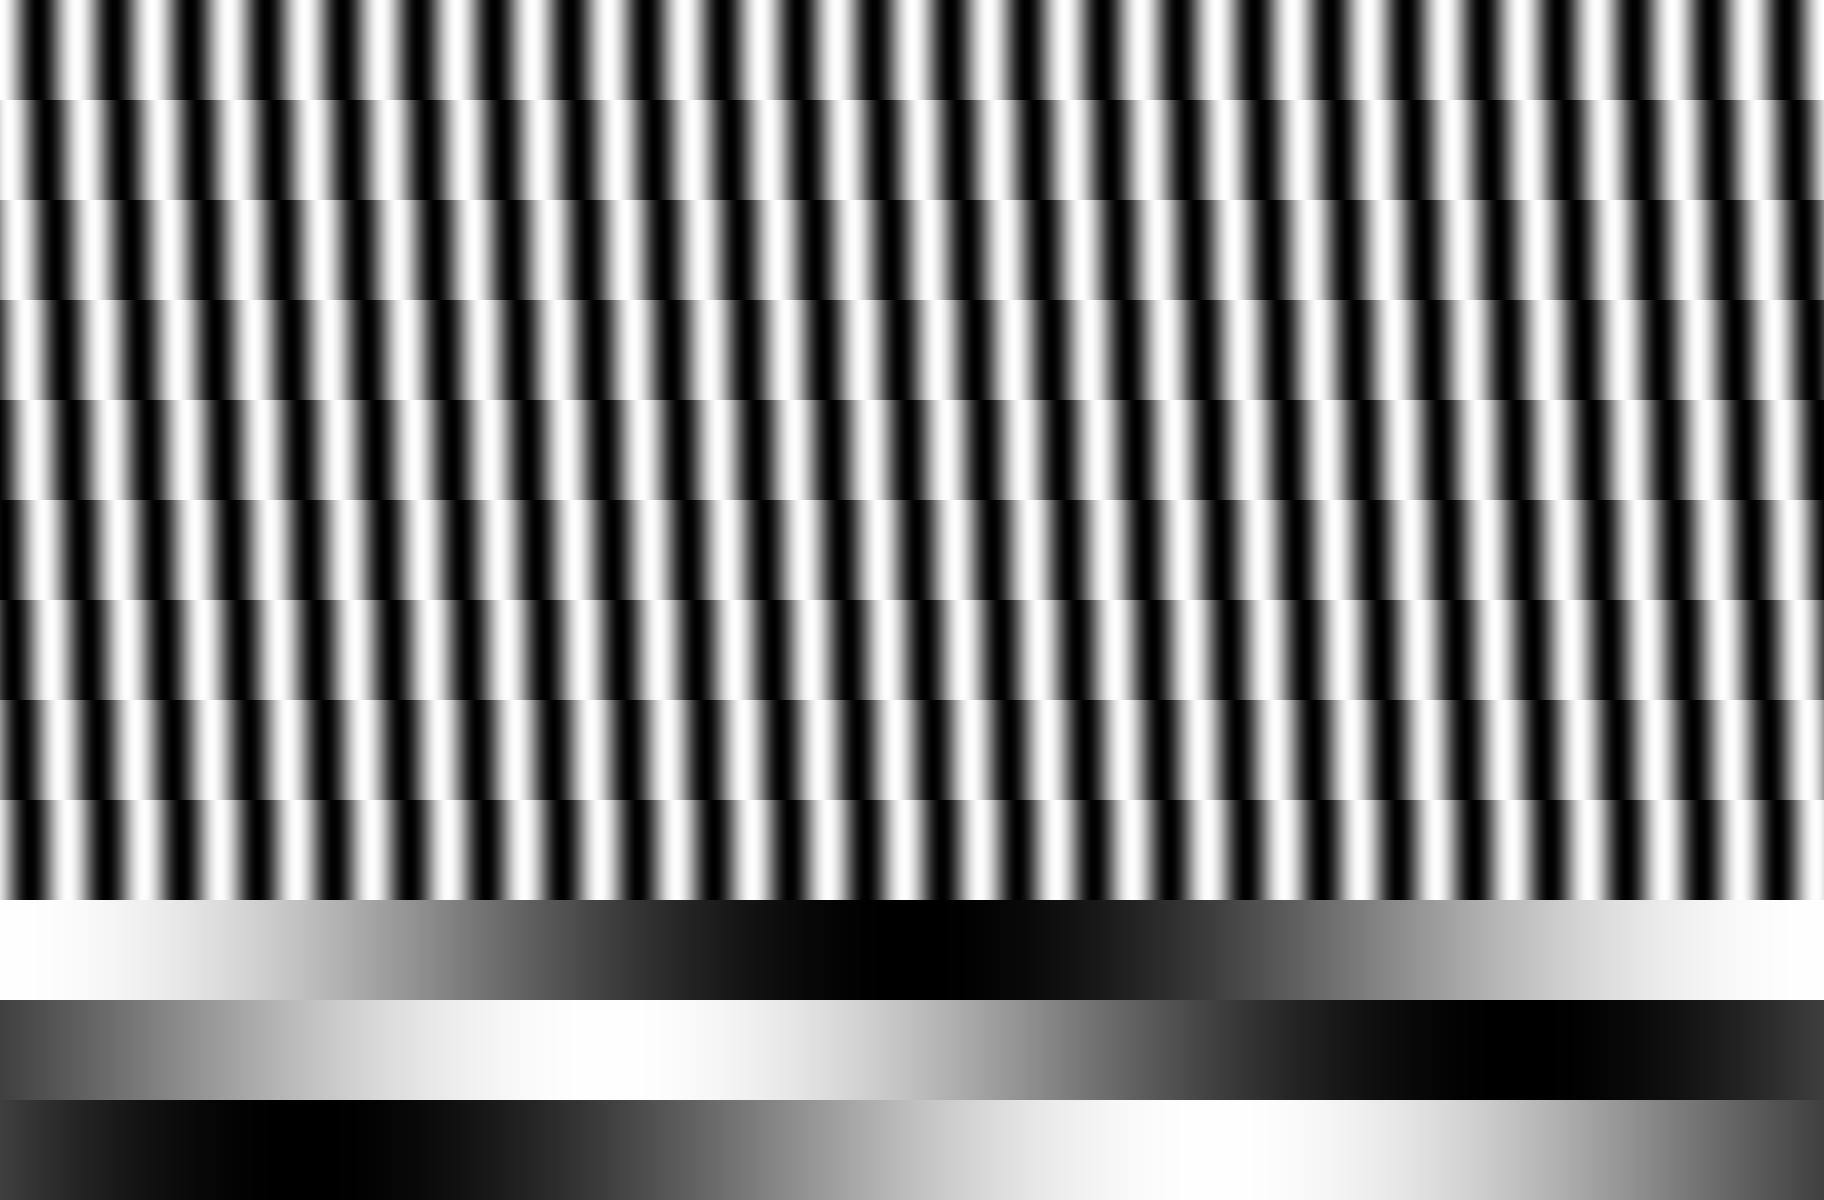
\includegraphics[width=0.49\linewidth]{figures/patterns_nstep}}
    \end{figure}
    \captionsetup[subfloat]{position=below, labelformat=empty}
    \vspace{-1cm}
    \begin{figure}
      \subfloat[Modulated Phase Shifting~\cite{chen2008modulated}]{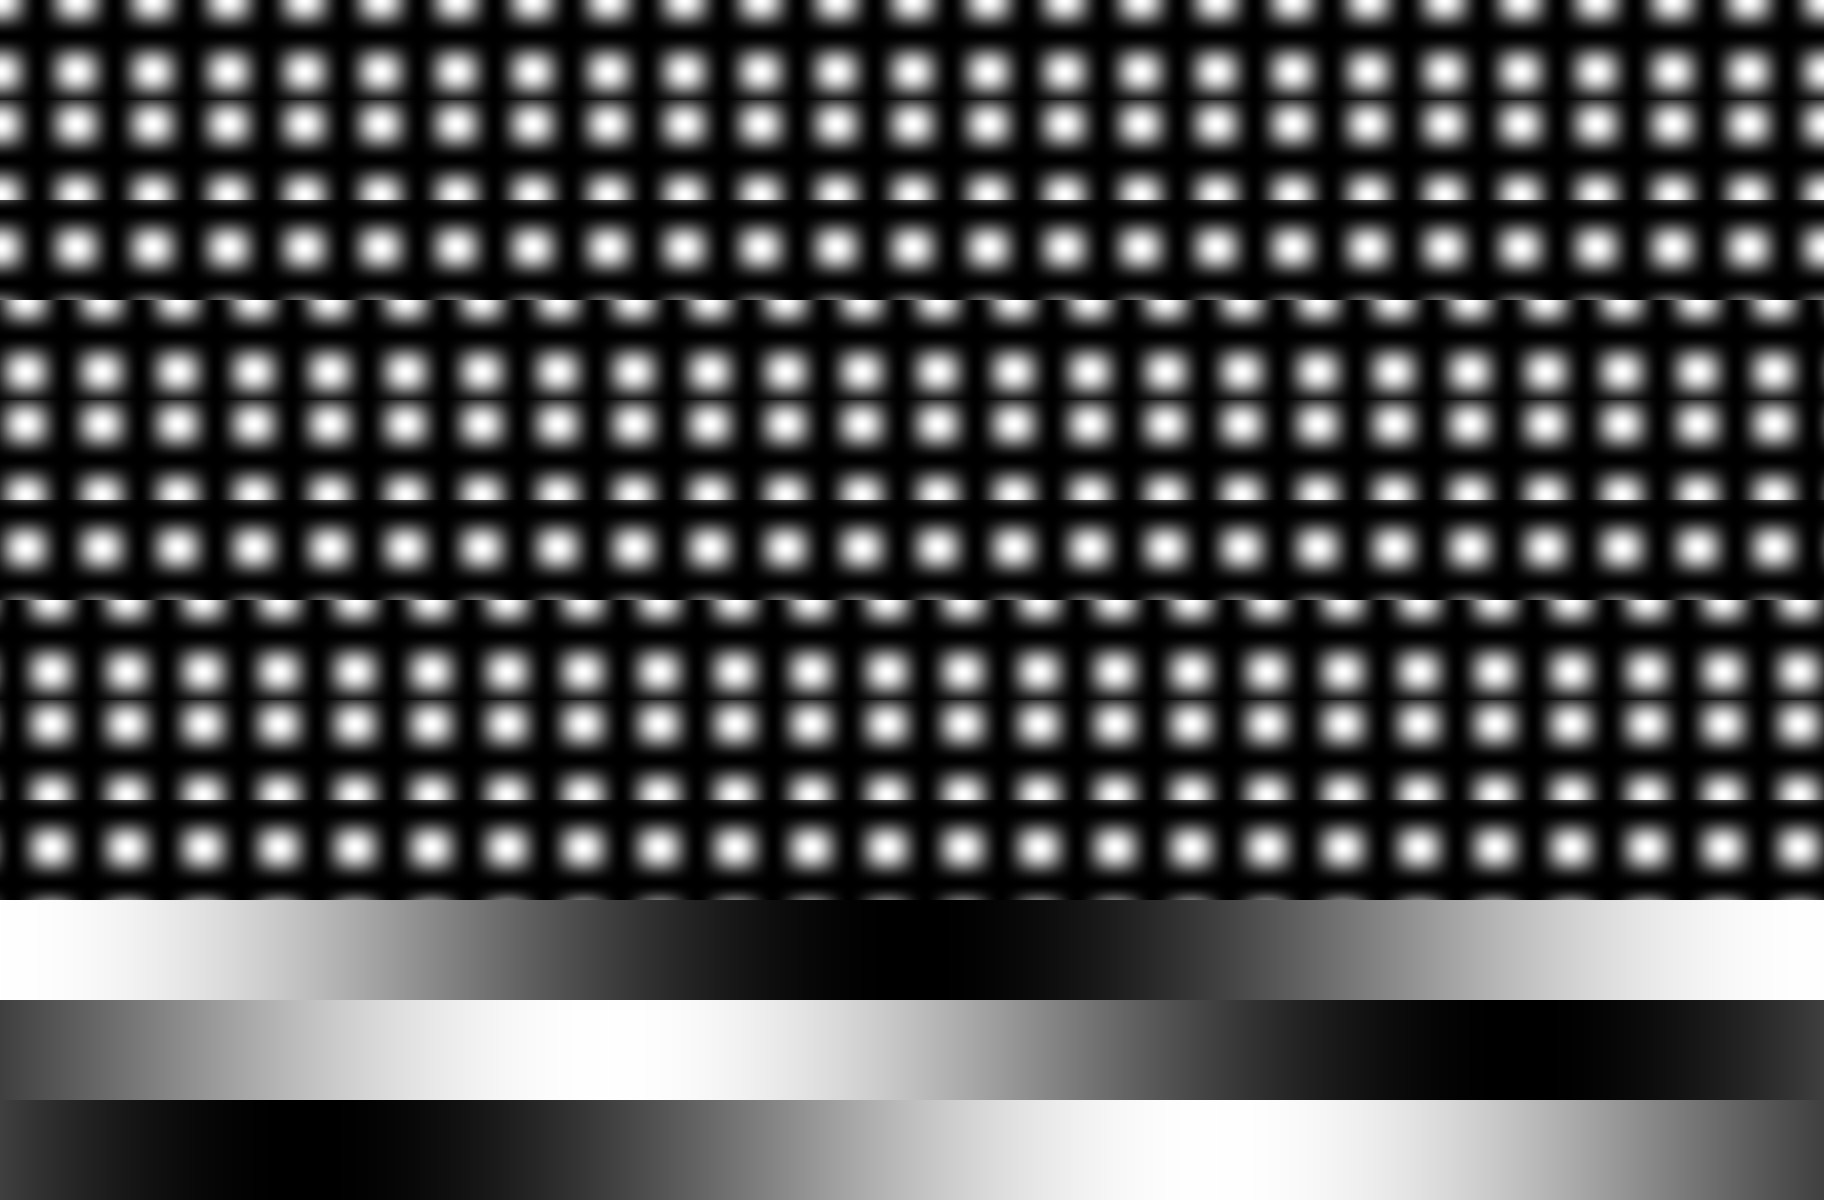
\includegraphics[width=0.49\linewidth]{figures/patterns_modulated}}\hfill
      \subfloat[Micro Phase Shifting~\cite{gupta2012micro}]{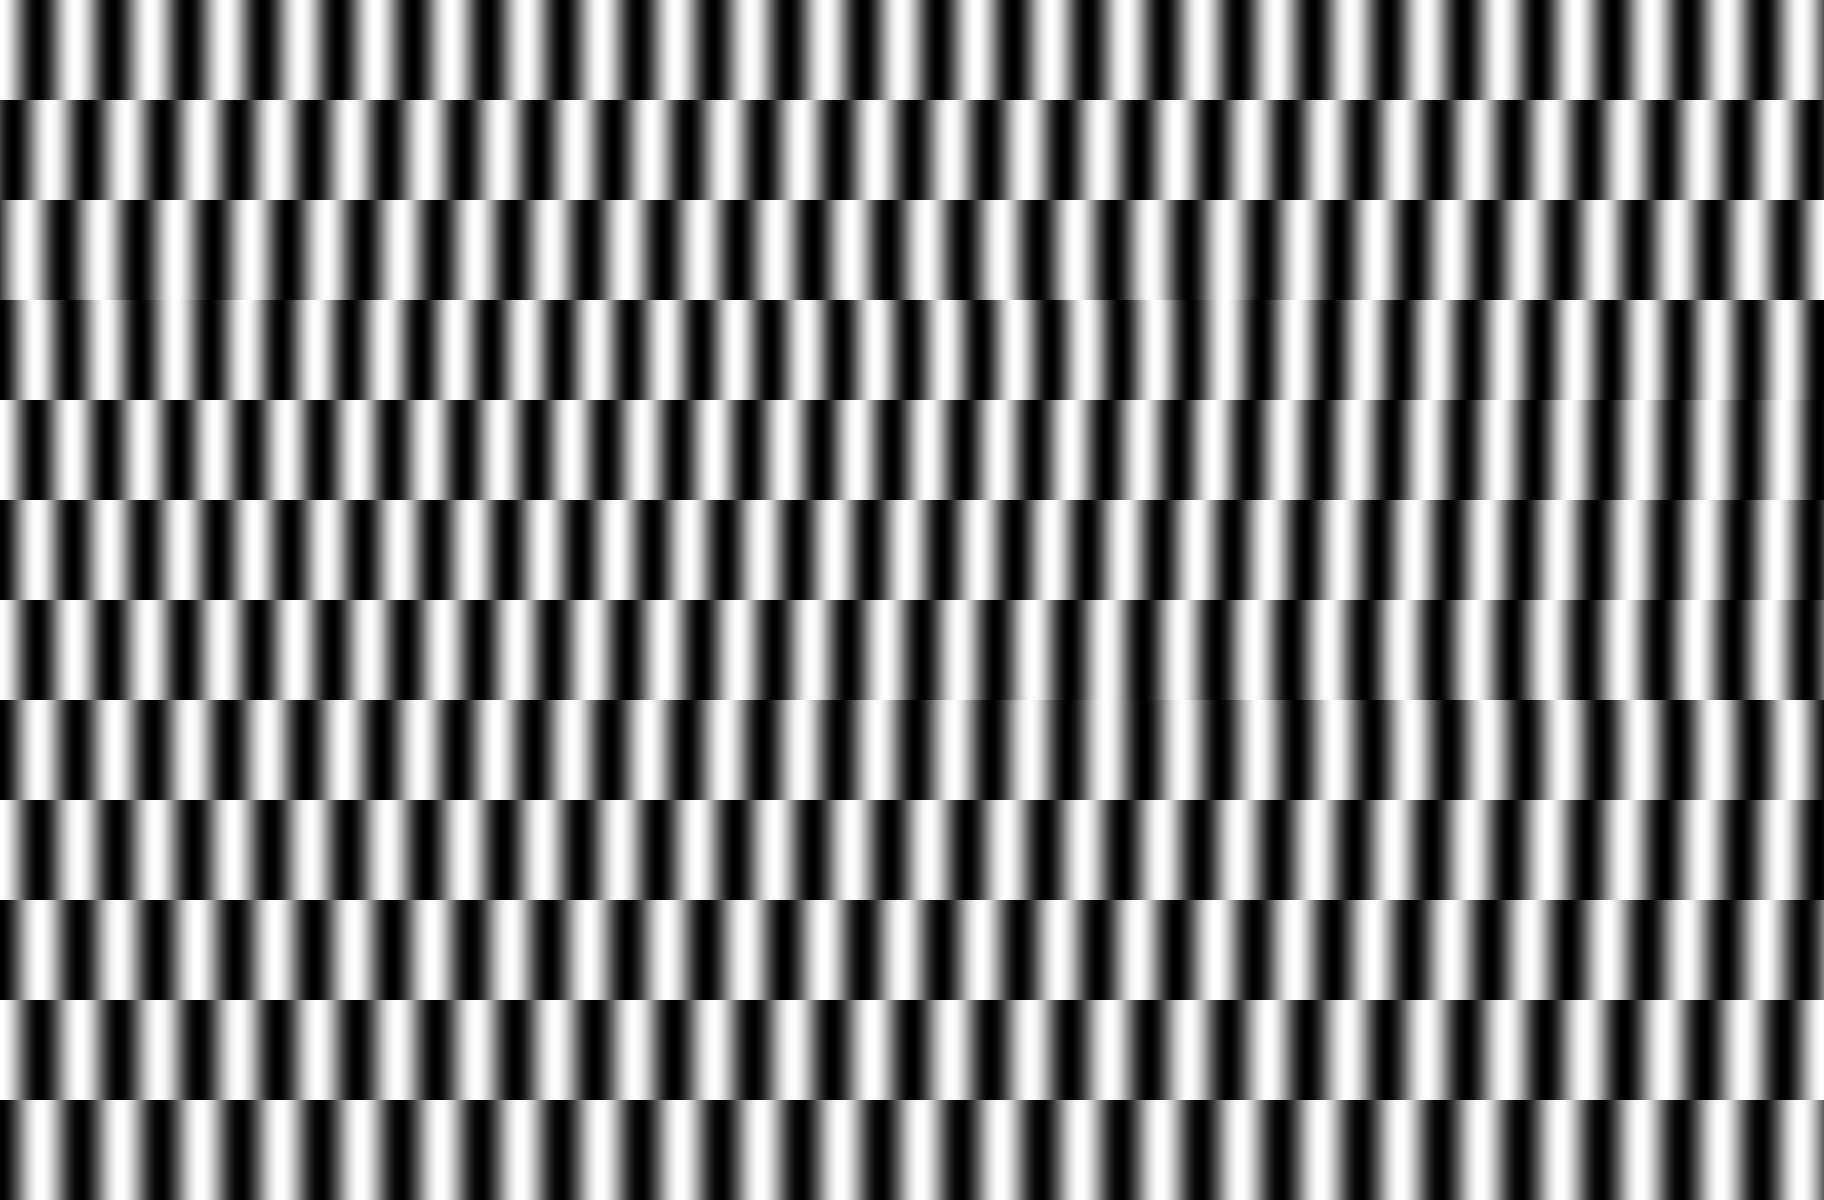
\includegraphics[width=0.49\linewidth]{figures/patterns_micro}}
    \end{figure}
  \end{minipage}
}
